\documentclass[a4paper,final,9pt]{article}

\usepackage{a4}
%\ueve-fonts-recommended:package[ascii]{inputenc}
\usepackage[T1]{fontenc}
\usepackage{colortbl}

\usepackage{graphicx}

\usepackage{xcolor}
\usepackage{url}
\usepackage{comment}
\usepackage{framed}
%\usepackage{savetrees}

\usepackage{times}


\usepackage{amsmath,amssymb,amsthm}

\title{Investigating particle swarm optimization}
\author{Edvard K. Karlsen}
\date {}

\begin{document}

\newcommand{\swarm}{\ensuremath{\mathcal{S}}}
\newcommand{\argmin}{\ensuremath{\text{argmin}}}
\newcommand{\argmax}{\ensuremath{\text{argmax}}}
\newcommand{\reals}{\ensuremath{\mathbb{R}}}
\newcommand{\vv}[1]{\ensuremath{\mathbf{#1}}}

\maketitle

\section{Introduction}

\subsection{Problem statement and solution overview}

My task was given as follows:
\begin{enumerate}
  \item Unders{\o}k `Particle Swarm Optimization' (PSO).  Det beskrives i
    mange AI b{o}ker, p{\aa} Wikipedia, osv.  Ingen mangel p{\aa} info.
  \item Implementere det fra scratch.
  \item Kj{\o}r din PSO p{\aa} 2 forskjellige TYPE problem - helst noen
    klassiske data problemer (som travelling            salesman, bare et
    eksempel) og minst 3 versjoner av hvert problem type.
  \item Skriv en 5-10 sider rapport om arbeidet, inklusivt resultater av dine
    kj{\o}ringer, analyse av dine resultater, osv.
\end{enumerate}

\noindent
I have studied and implemented a generic PSO algorithm from scratch in Python.
I discuss the underlying mathematical theory of the algorithm in
Section~\ref{sec:theory}. Further, I used my implementation to attack i) the
Single Machine Weighted Tardiness Problem, which is a NP-hard combinatorial
optimization problem, and ii) training of feed-forward neural networks for
(multi-class) classification. I experimentally confirmed PSO's optimization
ability for both these problems, and also did some emperical analysis of
parameters to investigate optimization performance.  I discuss the experiments
in Section~\ref{sec:anal1} and Section~\ref{sec:anal2}.  Finally, I reflect on the
work process and on my concluding impressions of PSO in
Section~\ref{sec:conc}.

Because there was no rigid `project description' text for this problem, I have
included much more background theory than in my previous reports, to provide
necessary context for my experiments. 

My main reference for this project has been Engelbrecht's excellent
textbook~\cite{engelbrecht}.


\section{Particle swarm optimization}
\label{sec:theory}
Particle swarm optimization is an iterative, stochastic optimization algorithm
inspired by the flocking of birds and schooling of fish; the main metaphor is
of social creatures moving in a swarm, with each creature's behavior dependent
both on personal preference and social influence.  PSO was first
described by Kennedy and Eberhart~\cite{kennedy95}. The algorithm sees a lot of
interest from the AI research community, who among other things tries to
formally investigate the optimization mechanisms of the algorithm; develop new
variants increasing performance (such as hybrid methods with other
bio-inspired methods); and develop special PSO incarnations to improve
performance on particular problems (such as TSP~\cite{wangtsp}). PSO has been
applied to a wide array of problems~\cite{poli}.

\subsection{Theory}
All PSO variants operate on an ordered set of \emph{particles}, each having a
\emph{position}, \emph{velocity}, and \emph{best position} vectors,
traditionally denoted $\vv{x}$, $\vv{v}$, and $\vv{p}$.  PSO operates by
`swarming', in discrete steps, the particles through a search space. 

Although there are
variations in the update rules between PSO algorithms, they always include a
`social component' -- which pulls each particle towards good positions known
collectively in the swarm, and a `selfish component' -- which pulls each
particle toward the best position it has visited.

\paragraph{gbest vs. lbest PSO}
Most texts distinguish between the \emph{global best} and \emph{local best}
PSO variants, traditionally named \emph{gbest} and \emph{lbest}.  The
difference is that in \emph{gbest} PSO, all particles always take the `social
step' towards the best among all seen positions by \emph{all} members of
swarm, while in \emph{lbest}, a particle only considers the best among the
members of its `neighboorhood'. However, gbest is clearly just the special
case of lbest with neighborhood size equal to the whole swarm's size, so we
can focus only on the lbest PSO, without loss of generality.

\paragraph{Notation}
For each PSO problems we discuss, let $g$ denote some function from
particle space to real numbers that is to be \emph{minimized}. Further, let
$\vv{x}_{i,t}$ denote the position of particle $i$ at time $t$, and assume
similar notation for velocities.  Also, let $\omega$, $\phi_p$, and
$\phi_g$ denote real numbers expressing the \emph{inertia}, \emph{personal
best acceleration factor}, and \emph{neighborhood best acceleration factor}
for the problem.  Finally, let's abuse notation and take $\vv{r}_p$ and
$\vv{r}_g$ as two vectors in particle space whose components are randomly and
uniformly sampled in $[0, 1]$ each time they appear in an equation.
\ \\

\noindent
With this notation, we can express the PSO update step of our implementation
as follows\footnote{Of course, our Python code is much more
`imperative-looking' than this, for example, we store best positions instead
of re-computing them all the time. However, the mathematical formulation in
the text helps to avoid ambiguity.}:
\begin{align*}
  \vv{v}_{i,t+1} &= 
    \omega \vv{v}_{i,t} 
    + \phi_p \vv{r}_p (\vv{p}_{i,t} - \vv{x}_{i,t})
    + \phi_g \vv{r}_g (\vv{g}_{i,t} - \vv{x}_{i,t}) &
    \text{Velocity update} \\
  \vv{x}_{i,t+1} &= \vv{x}_{i,t} + \vv{v}_{i,t} & \text{Position update} \\
  \ \\
  \vv{p}_{i,t} &= \argmin~g~\{~\vv{x}_{i,u}~|~u~\in~[0,~t]~\} 
    & \text{Personal best position} \\
  \vv{g}_{i,t} &= \argmin~g~\{~\vv{p}_{j,t}~|~j~\in~\text{neighbor-ids}(i)~\} 
    & \text{Neighborhood best position} 
\end{align*}
~~~~~~~~~where $\text{neighbor-ids}(i) =
\{~i,~i+1,~\ldots,~i+\textsc{neighborhood-size}~\}$
\ \\

\noindent
The update equations are the most important formality needed to describe our
implementation, but, the devil is in the details and there are many
other smaller aspects of the algorithm that we could have discussed in depth.
Most important are \emph{initialization}, \emph{velocity/particle clamping},
\emph{inertia reduction}, and \emph{stopping criteria}. These are however more
problem-specific, and we therefore discuss them in context of our experiments
(Section~\ref{sec:anal1}~and~\ref{sec:anal2}).

\subsection{Digression: The nature of the lbest PSO}
It's interesting to philosophise about inter-neighborhood communication in the
lbest PSO.  Clearly, with neighborhoods comes an element of `information lag'
in the swarm. A swarm-global best position, call it $p$, known only in one
neighborhood, may require many steps before it becomes known to a distant
neighborhood; with the typical definition of neighborhood membership, a local
best can propagate to at most one new particle in each iteration.  This has
two important consequences, one positive and one negative: First, it enables
other neighborhoods to focus on \emph{exploring} their local bests, which may
lead to even better positions than $p$, and hence help in avoiding premature
convergence to non-global optima. Second, if $p$ is a useful position that
should be heavily \emph{exploited}, it may take (potentially, \emph{much})
longer time to direct the swarm's attention towards it.  Ideally, PSO should
be tuned so as to balance these consequences for the best results.  With the
\emph{Unified PSO}~\cite{unified}, Parsopoulos and Vrahatis propose
mitigating this problem by having the swarm gradually focus more on global
information (and less on neighborhood information) during the PSO run.

\subsection{Investigating the PSO}
A typical evaluation of an optimization algorithm includes an empirical
comparison with an alternative algorithm known from the literature, and the
typical argument is that the proposed algorithm performs better, in some
sense, than another method on some benchmark problems. For example, to
demonstrate PSOs quality as a training algorithm for feed-forward artificial
neural networks, a comparison with traditional backpropagation would be
natural.  

One can also `compare it with itself', and study how PSO's performance depends
on its many configuration options. Among those are:
\begin{enumerate}
  \item The number of particles used.
  \item The value of the acceleration constants $\omega$, $\phi_p$, and
    $\phi_g$.
  \item Whether to use position and/or velocity clamping, and if so, its
    rules.
  \item Whether to use inertia dampening, and if so, the inertia dampening
    rules.
  \item The swarm structure. (gbest/lbest, neighborhood size, alternative
    swarm topologies.)
\end{enumerate}

In planning this project, I quickly concluded that doing a truly rigorous
investigation of the PSO's workings could pose too much of a challenge; there
are simply too many variables to look at. Therefore, I decided that I had to
choose more modest goals, and after some pondering I settled on the following:

\begin{framed}
  \textsc{experiment goals}
  \begin{enumerate}
    \item Demonstrate PSO's optimization ability on two hard problems:
      (i) SMTWTP and (ii) training of feed-forward ANNs.
    \item For the SMTWTP experiment: Demonstrate how a problem-specific hybrid method can
      improve PSO's performance.
    \item For the ANN training experiment: Investigate the dependence between
      number of fitness evaluations and solution quality.
   \end{enumerate}
\end{framed}


\section{Application: Single Machine Total Weighted Tardiness}
\label{sec:anal1}

\subsection{Discrete and combinatorial PSO}
PSO is in its traditional form directly applicable only for real-valued
problems, and no one-size-fits-all method for adapting it to discrete-valued
and combinatorial problems have yet been discovered. 
PSO-variants that perform well on discrete/combinatorial problems often
include some creative variation of the particle data structure, and
alternative definitions of the position and velocity update equations.  

Within the limited scope of this project, I opted to find a combinatorial
optimization problems that could be solved by applying a less `intrusive'
method: Running the traditional continuous PSO, but applying some mapping from
the search domain to the discrete problem domain.

One hard problem that has been convincingly attacked~\cite{tardiness} in this
way is the Single Machine Total Weighted Tardiness Problem. My solution is a
basically a small-scale clone of Tasgetiren et al.'s approach.

\subsection{Theory}
The objective is to schedule a set of jobs given per-job
\emph{processing times}, \emph{due times}, and \emph{weights}, such that the
weighted sum of per-job \emph{tardiness} -- a penalty measure for overdue jobs
-- is minimized. Two constraints apply: (i) only a single machine can be used
and (ii) jobs cannot be interleaved. Let's formalise this:

\begin{framed}
  \textsc{single machine total weighted tardiness problem}
\\
\ \\
Let $\textbf{P}$, $\textbf{D}$, and $\textbf{W}$ be three ordered sets each
containing $n$ non-negative real numbers. Call a permutation of the integers
$[0, n-1]$ a \emph{schedule}.  The goal is to find a schedule minimizing the
\emph{total weighted tardiness}:
$$
\text{twt}(p) = \sum_{i=1}^{n}~\max~\{~\textbf{W}_i(S(p, i) + 
                  \textbf{P}_i - \textbf{D}_i),~0~\} 
$$
where $S(p, i)$ denotes the \emph{starting time} of the $i$th job\footnote{Our
definition of $\textbf{S}_i$ does not allow pauses between jobs, but, clearly,
removing a pause can never increase the total tardiness of a schedule, so we
do not need to consider schedules with pauses.} with respect to permutation
$p$, that is $\textbf{S}_i = \sum_{j=1}^{i-1} \textbf{P}_{p_j}$.
\end{framed}

To map the real-valued search positions into interpretable schedules, we use a
simple relation from vectors to integer permutations named the \emph{SPV
rule}~\cite{tardiness}.

\begin{framed}
\textsc{spv rule}
\\
\ \\
For a $k$-element vector $\vv{x} \in \reals^k$, let $\text{spv}(\vv{x})$
denote the permutation $p$ of the integers $[0,~k-1]$ such that $p_i$ is the
index of $i$th largest element in $\vv{x}$. If there is ambiguity because of
similar elements, always select the element with the lowest index.
\end{framed}
\noindent
For example, $\text{spv}([1,0,2]) = [1,0,2]$, and $\text{spv}([0,4,0.1,2.3])
= [0,2,3,1]$.

\paragraph{Augmentation: Local search}
In addition to implementing this `standard' PSO, we did like Tasgetiren et al.
and implemented an option to use a local search component as part of the
optimization. This is a commonly seen augmentation of
PSO which primarily is used to increase exploitation
potential~\cite{engelbrecht} (although PSO is good at finding high-quality
solution spaces, it can struggle with locating the precise optimas). 
Specifically, we implemented functionality for client code to pass in a
`per-step manipulation function' which then is called from the PSO main loop
after each position update. The specific manipulation function we used is
given below, as Python-style pseudo code.
\begin{verbatim}
function local_search(p):
  in 10% of cases do:
    orig_sol = p.pos
    best_score, best_pos = eval_fitness(orig_sol), orig_sol
    repeat fifteen times:
        v, w = random indices
        s = orig_sol
        s[v], s[w] = s[w], s[v]
        score = eval_fitness(s)
        if score < best_score:
            best_score, best_pos = score, s
    p.pos = best_pos
\end{verbatim}
This is a simple search trying fifteen random swaps of elements in the
considered particles position vector, and leaves it in the best
state\footnote{My rough estimates showed that the local search found better
positions than the start in approximately $\frac{1}{3}$ of all cases}. Also,
local search only runs one out of ten times.

We call the augmented PSO `PSO+LS', and the standard PSO `PSO'.


\subsection{Experimental setup}
For a $k$-job problem, we configured PSO as follows (see \texttt{smtwtp.py}):
(The parameters were selected through trial and error, using values reported
by Tasgetiren et al. as guidelines. 80 particles may seem a lot in
`traditional' PSO sense, but many-particle configurations are routinely used
in high-dimensionality problems like this.)

\noindent
\line(1,0){368}
{\footnotesize
\begin{description}
  \item[Domains:] $D = \{ x \in \reals^k | -1 \leq x_i \leq 1 \}$
  \item[Initial positions:] [Uniform and randomly sampled subset of $D$]
  \item[Optimization goal:] Minimize $g = \text{twt} \circ \text{spv}$
  \item[Velocity clamping:] Yes. $v_i$ is clamped within $[-8, 8]$ before each
    position update. 
  \item[Position clamping:] No. \footnote{For most PSO-problems, position
    clamping is a strictly necessary to ensure solution integrity. However,
    when using SPV, there is no formal need to restrict the domains, and
    performance seems to improve greatly when we do not.}
  \item[Initial inertia:] $\omega = 1$ 
  \item[Trust coefficients:] $\phi_p = 1.5$, $\phi_g = 1.5$
  \item[Inertia decrement rule:] Multiply by 0.99 before each iteration, as
    long as the current inertia is greater than $0.6$.
  \item[Number of particles:] 80
  \item[Neighborhood size:] 5
\end{description}
}
\noindent
\line(1,0){368}

\noindent
We used as benchmark problems the first 20 of the 40-job SMTWTP instances in
the well-known
OR-Library\footnote{\url{http://people.brunel.ac.uk/~mastjjb/jeb/info.html}}.
We ran `standard' PSO and PSO+LS eight times on each problem (for a total of
$10*8*2 = 160$ evaluations), and computed the minimum, maximum, arithmetic
mean, and standard deviation of the solution scores for each run-of-eight.
Each algorithm was allowed to compute for forty seconds on a modern laptop.

Arguably, eight evaluations per case is \emph{far} too low a number to allow
rigorous statistical arguments, but we can use the results to do some
careful analysis.\footnote{The reason that I did not run more tests per case
is simply that running the experiments took too much time, I had to
get on with data analysis and writing\ldots}


\subsection{Results}

\begin{table}[h!]
  \label{tab:res1}
  \begin{center}
    \begin{tabular}{|c|c|c|c|c|c|c|}
      \hline
      $\textbf{\#}$ & $\mathbf{Alg.}$ & $\mathbf{g}_\text{opt}$ & $\mathbf{g}_\text{$\min$}$ & $\mathbf{g}_\text{avg}$ & $\mathbf{g}_\text{$\max$}$ & $\mathbf{g}_\text{$\sigma$}$ \\
\hline
\textbf{1} & \textsc{pso} & 913 & 930 & 949 & 956 & 11.27\\
\hline
\rowcolor{pink}  & \textsc{pso+ls} & 913 & 913 & 932 & 956 & 15.36\\
\hline
\scriptsize{~}\\
\hline
\textbf{2} & \textsc{pso} & 1225 & 1264 & 1377 & 1535 & 69.33\\
\hline
\rowcolor{pink}  & \textsc{pso+ls} & 1225 & 1225 & 1232 & 1263 & 13.11\\
\hline
\scriptsize{~}\\
\hline
\textbf{3} & \textsc{pso} & 537 & 573 & 573 & 573 & 0.00\\
\hline
\rowcolor{pink}  & \textsc{pso+ls} & 537 & 537 & 568 & 573 & 11.92\\
\hline
\scriptsize{~}\\
\hline
\rowcolor{pink}\textbf{4} & \textsc{pso} & 2094 & 2094 & 2148 & 2307 & 78.20\\
\hline
\rowcolor{pink}  & \textsc{pso+ls} & 2094 & 2094 & 2094 & 2094 & 0.00\\
\hline
\scriptsize{~}\\
\hline
\rowcolor{pink}\textbf{5} & \textsc{pso} & 990 & 990 & 990 & 990 & 0.00\\
\hline
\rowcolor{pink}  & \textsc{pso+ls} & 990 & 990 & 990 & 990 & 0.00\\
\hline
\scriptsize{~}\\
\hline
\rowcolor{pink}\textbf{6} & \textsc{pso} & 6955 & 6955 & 7029 & 7484 & 173.17\\
\hline
\rowcolor{pink}  & \textsc{pso+ls} & 6955 & 6955 & 6955 & 6955 & 0.00\\
\hline
\scriptsize{~}\\
\hline
\rowcolor{pink}\textbf{7} & \textsc{pso} & 6324 & 6324 & 6493 & 6571 & 105.86\\
\hline
\rowcolor{pink}  & \textsc{pso+ls} & 6324 & 6324 & 6369 & 6571 & 84.84\\
\hline
\scriptsize{~}\\
\hline
\rowcolor{pink}\textbf{8} & \textsc{pso} & 6865 & 6865 & 6876 & 6927 & 21.26\\
\hline
\rowcolor{pink}  & \textsc{pso+ls} & 6865 & 6865 & 6865 & 6865 & 0.00\\
\hline
\scriptsize{~}\\
\hline
\rowcolor{pink}\textbf{9} & \textsc{pso} & 16225 & 16225 & 16530 & 16758 & 180.42\\
\hline
\rowcolor{pink}  & \textsc{pso+ls} & 16225 & 16225 & 16225 & 16225 & 0.00\\
\hline
\scriptsize{~}\\
\hline
\textbf{10} & \textsc{pso} & 9737 & 9741 & 9796 & 9903 & 61.85\\
\hline
\rowcolor{pink}  & \textsc{pso+ls} & 9737 & 9737 & 9743 & 9771 & 10.44\\
\hline

    \end{tabular}
  \end{center}
  \caption{Experimental results from SMTWTP} 
\end{table}

The results are shown in Table~\ref{tab:res1}. The column
$\mathbf{g}_\text{opt}$ gives the known optimum values for each instance.  The
rows colored red/pink are rows where at least one optimization run reached the
known global minimum.

\subsection{Discussion}
Interpreting the results can be a bit challenging; although reaching the known
optimum is `excellent' by any interpretation, it is not immediately clear how
good or bad a non-optima like 956 (cf. the minimum, 913) for the first problem
instance is. Reaching the solution with 5-10 \% error can be very good, if the
problem space is complex, and most areas contains solutions that are
magnitudes larger than the optimum.  To make sense of this, one option would
be to compare the results with those obtained by for example a well-known
greedy solution to the problem. Still, there are many interesting observations
we can make from our data.

Standard PSO find the optimum at least once in eight runs for six out of ten
problems. Out of these, there is one problem (\# 5) that the algorithm always
solves to the optimum.  Problem 3, on the other hand, seems to be especially
hard for standard PSO.  All runs end up at 573, while the true optimum is 537.
From manual analysis of the runs we believe that the 573 optimum lays in a
large initially good-looking region of the search space, from which it is hard
to reach the global optimum.  Also, the topology of the global optimum may be
such that PSO are not able to exploit it effectively. (From inspection, it
seems like the swarm is not able to find the 537 global optimum once the
misleading 573 optimum has been visited, even when we stretch all
configuration parameters to reduce the convergence rate.)

From the minimum and maximum values and the standard deviations we see that
standard PSO is quite robust on most problems, with a multiple of
hundred units as the typical difference in total weighted tardiness.
However, there are outliers, such as 1535 for Problem 2, where the global
optimum is 1225. A lesson to draw from this is that for real-world problems
several PSO runs should be used, to increase the confidence in the quality of
the solution.

The results strongly suggests that adding stochastic local search to the
algorithm increases robustness. First, all of the PSO+LS runs are able to
reach the global optimum. Second, PSO+LS solves not one but five out of ten
problems perfectly for every run. Third, the maximum solutions are usually
notably better than those for standard PSO. Our conclusion is that weaving local
search into the algorithm increases performance and accuracy. 

Taken as a whole the results indicate that our PSO is able to optimise for the
SMTWTP, but that convergence to global optima can not be guaranteed. However,
helping the algorithm with a simple local search algorithm to increase
exploitation power makes the algorithm more robust.  


\section{Application: Artificial Neural Network Training}
\label{sec:anal2}
{ \footnotesize \emph{(I must admit up-front that I have not done any
programming with ANNs before this, so there might be some errors in my
understanding.  My goal is to show the gist of how PSO is used to train
ANNs.)} }
\vspace{5pt}

\noindent
Another interesting PSO application is training of artificial neural networks.
Typically, the researcher proposes a network structure, and lets the PSO
search in weight space, so that each particle corresponds to one specific
neural network. The fitness measures is then taken as the induced network's
performance on a training set. (More advanced PSO variants have been proposed
to optimise both the weights and architecture of ANNs, by for instance
by Carvalho and Ludermir~\cite{carvalho}.)

We investigate optimization performance for feed-forward ANNs with a single
hidden layer, bias, and the traditional sigmoid activation function for the
hidden and output layer nodes. We use one output node per class, and code the
expected output vector for an instance with, say, correct class 2 as
$[0,0,1]$. The network's classification of an input instance is taken as the
index of the maximum value in the output vector. Such a network has $N = $ [\#
Inputs] $\times$ [\# Hidden] + [\# Hidden] $\times$ [\# Outputs] weights
(counting bias as an extra input), and the PSO therefore searches in
$\reals^N$.

While there of course are more intelligent error measures
available\footnote{For binary classification problems, it's clear that coding
the output with one output node, and using mean squared error as a fitness
measure is straightforward. However, I did not achieve good results when
testing MSE variants for my multi-class setup. This probably stems from a
problem located between the chair and the computer screen. That is, my lack of
experience with ANNs\ldots} for
multi-class ANN training, we opted to use only a very basic error measure, the
percentage of mis-classified instances, which for a weight configuration
$\mathbf{w}$ and a data set $\mathbf{X}$ can be defined as:
$$
\text{err}(\mathbf{w}, \mathbf{X}) = 
  \frac{ |\{ \text{c}(\mathbf{w}, \mathbf{x}) \neq a~|~(\mathbf{x}, a) \in
        \mathbf{X} \}| }
       {|\mathbf{X}|}
$$
where $\text{c}(\mathbf{w}, \mathbf{x})$ denotes the classification of
instance $x$ with respect to the weights.

\clearpage

\subsection{Experimental setup}
For a $N$-coefficient ANN training problem, we configured PSO as follows (see
\texttt{ann.py}):

\noindent
\line(1,0){368}
{\footnotesize
\begin{description}
  \item[Domains:] $D = \{ x \in \reals^N | -8 \leq x_i \leq 8 \}$
  \item[Initial positions:] [Uniform and randomly sampled subset of $D$]
  \item[Optimization goal:] Minimize $g = \text{err}$ 
  \item[Velocity clamping:] No. 
  \item[Position clamping:] Yes.   
  \item[Initial inertia:] $\omega = 1$ 
  \item[Trust coefficients:] $\phi_p = 2.4$, $\phi_g = 2.4$
  \item[Inertia decrement rule:] Multiply by 0.99 before each iteration, as
    long as the current inertia is greater than $0.6$.
  \item[Number of particles:] 60
  \item[Neighborhood size:] 5
\end{description}
}
\noindent
\line(1,0){368}

\noindent
These parameters were selected through trial and error (a more ambitious and
`correct' option could be to run a meta-optimiser). It's worth commenting on
the clamping rules: When using position clamping, and gradually reducing
inertia, it is not strictly necessary to use velocity clamping, and in fact it
may often reduce search quality. Also here, 60 particles is suitable for this
high-dimensionality problems. 

We ran the algorithm on three classification problems from the UC Irvine data
set repository:
\begin{description}
  \item[Iris] Iris is `perhaps the best known database to be found in the
    pattern recognition literature', and a standard benchmark problem for any
    classifier. The data set contains 150 instances and encodes four attributes
    and three classes (with 50 instances of each). Two of the three classes
    are linearly separable, while one is not.

  \item[Seeds] This data set contains `measurements of geometrical properties
    of kernels belonging to three different varieties of wheat'. The data set
    consist of 210 instances with 7 attributes each, and has three classes.

  \item[Glass] Another well-known data set. Consists of 214 instances,
    encodes 10 attributes, and has 7 classes. Glass is a notoriously hard data
    set for classifiers, with error rates around 30\% commonly reported. 
\end{description}

\noindent
We used trial and error, with tips from the Neural Network
FAQ\footnote{\url{ftp://ftp.sas.com/pub/neural/FAQ.html}}, to select the
number of hidden units for each problem. We initially tested 10-15 unit
configurations, but in the end we settled on 3 hidden units for Iris, 5 hidden
units for Seeds, and 5 hidden units for Glass. Although these sizes have been
selected with care, \emph{sub-optimal network architecture choices is a
notable threat to validity of our results and the conclusions drawn from
them}.

Our objective for these experiments was to show how classification performance
depends on the number of fitness evaluations, that is, the number of tests of
weight configurations. To do this, we evaluated training performance for each
data set for various configurations of evaluation counts ranging from 100 to
30000 (see \texttt{ann.py}). For Iris and Seeds we performed 25 PSO runs for
each maximum count; for Glass we performed 10 PSO runs per maximum count
(probably due to the quadratic growth of the network computation requirements,
computing for Glass took significantly longer than for the other sets).
For each run, the data set was randomly split into training and test sets,
with $\frac{3}{5}$ of instances going into the training set.

\subsection{Results and discussion}

We now present and discuss the experimental results. In each figure below, we
plot mean training and testing accuracy on each data set. In addition, each
figure includes a scatter plot (red dots) showing \emph{all} classification
performances.  The intention of the scatter plot is to give a rough indication
of robustness.

\subsubsection{Iris}
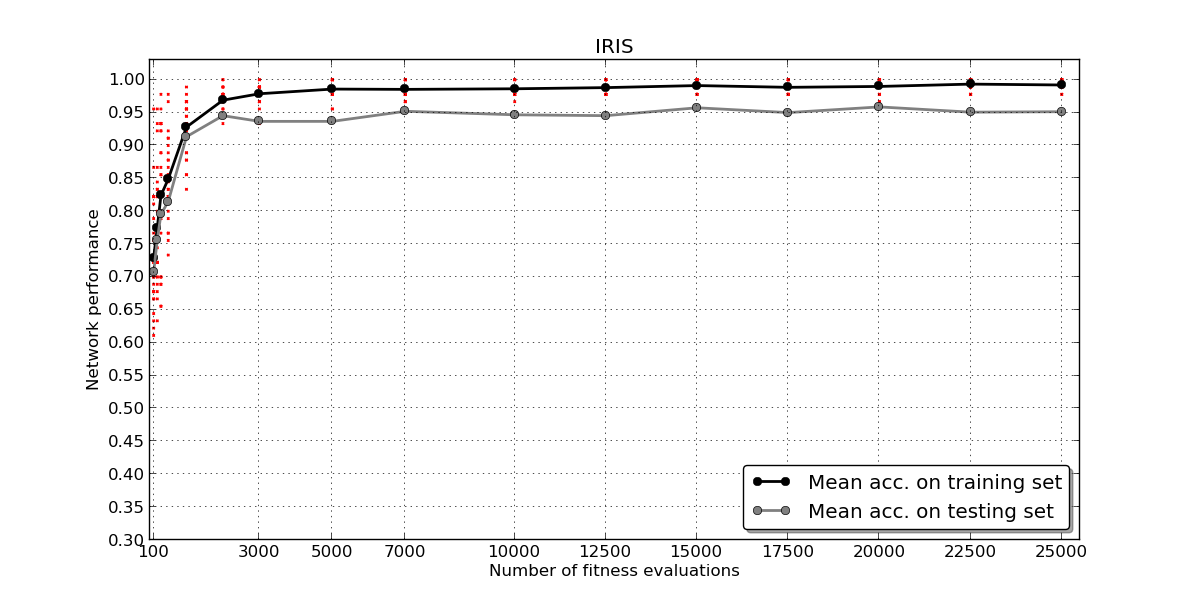
\includegraphics[width=0.99\textwidth]{iris-ann-performance.png}

\noindent
Evidently, PSO performs very well on the Iris set. The scatter plot shows that
the best runs reach 100\% training accuracy with about 2000 evaluations, and
that the testing accuracy always is in the upper part of the 95-100 \%
region as long as we use more than 3000 runs. Mean testing accuracy reaches
95\% for 2000 evaluations, and is not significantly improved with more
evaluations (in fact, at 3000 and 5000 evaluations, mean testing acc. is about
93\%). Our conclusion is that PSO performs strongly and robustly on this data
set. The robustness is evident from the scatter plot: the results of single
runs tend very close to the mean.

\subsubsection{Seeds}
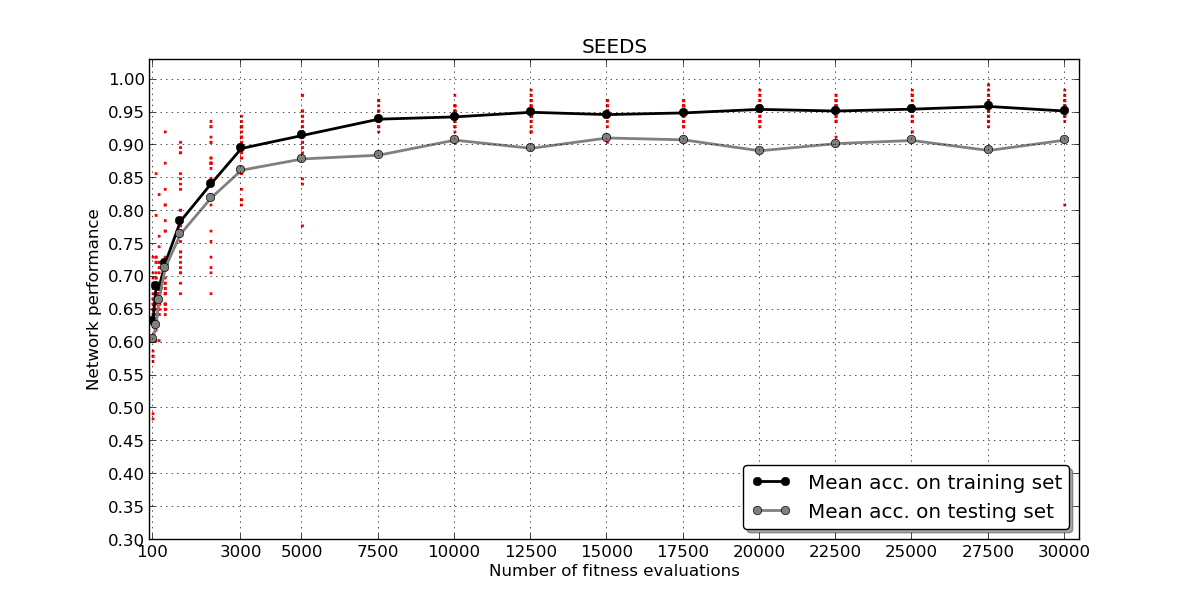
\includegraphics[width=0.99\textwidth]{seeds-ann-performance.png}

\noindent
In comparison with performance on Iris, PSO requires more iterations to
stabilise on the Seeds data set. One probable cause is the larger search
space: For Seeds we use both more input and hidden nodes than with Iris. Mean
training accuracy increases steadily up to 10000 evaluations, where it levels
out at about 95\% level. Mean testing accuracy also levels out around 10000
evaluations, and subsequently fluctuates around the 90\% point, with no clear
sign of overfitting.  It's evident that the biggest gains from adding fitness
evaluations appears in the range up to 10000 evaluations. After that point,
there are no clear changes in performance. This can either mean that the
classifier has reached an optimal area of the search space, or, more probably,
that PSO is not able to put the additional fitness evaluations to use.
(Clearly, a search with a high bound on the number of evaluations should be
configured to converge slower than a search with stricter constraints.)

The algorithm does not perform
very robustly: at 12500 evaluations, we see that the span between the minimal
and maximum solutions is about 10\%. Also, there are a few low-performance
outliers, the most extreme one being the minimal result of the
30000-evaluation runs, at about 82\%. These outliers indicate a
danger of early convergence to sub-optimal locations of the search space.
Still, the scatter plot indicates that many runs perform strongly ($\geq
97\%$), and thus a practitioner could probably extract a very strong
classifier by adding a validation set [for a (\emph{train}, \emph{validation},
\emph{test})-triple] and selecting the best of several strong-performing
classifiers found by repeated runs.

\subsubsection{Glass}
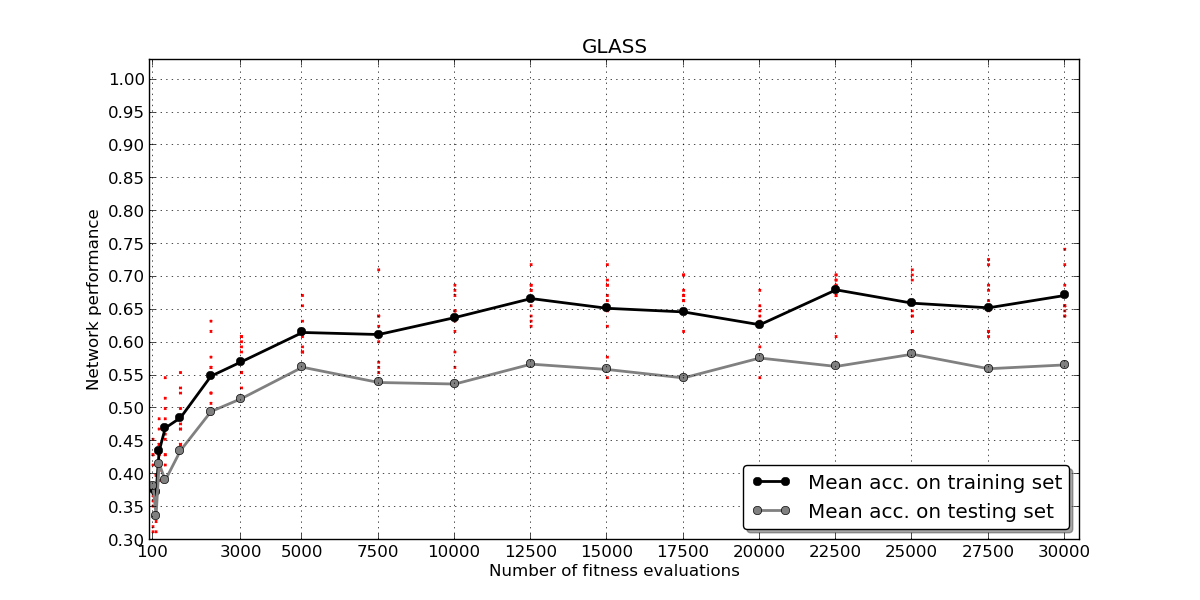
\includegraphics[width=0.99\textwidth]{glass-ann-performance.png}

\noindent
As noted, Glass is a hard data set for most classifiers\footnote{We also saw
this when we used it in investigate boosting for the previous AI programming
project.}, and our PSO algorithm also struggles with achieving higher training
accuracy than
about $65\%$. The strongest result is the maximum training accuracy of the
30000-evaluation run, at nearly $75\%$. It seems that optimization performance
levels out around 10000 evaluations. 
From the scatter plot it is evident that PSO's performance on Glass is the
least robust. At 15000 evaluations the difference in training
accuracy between the best and worst run is more than $15\%$. This can indicate
early convergence to sub-optimal locations of the weight space.

Also here, using repeated runs and a validation set could help us extract
powerful classifiers even though mean performance is not impressive. Already
at 7500 evaluations there are runs with more than $70\%$ training accuracy. 

Given the hardness of this particular data set, we are satisfied with PSO's
performance, but, it would be interesting to investigate techniques to control
convergence and make the algorithm more robust for this and other hard
problems.


\section{Concluding remarks}
\label{sec:conc}
In this text we have reported on my experience implementing and experimenting
with particle swarm optimization. We have shown that PSO can be used
effectively for optimisation of two hard problems.
\ \\

\noindent
Doing this project has been challenging for several reasons. First, as I was
the only student working on this project, I did not have the usual arena for
discussing theory and gotchas with other students in the course, which has
been very helpful on the previous projects\ldots Second, as with many AI
algorithms, the devil is in the detail. Unlike implementing Edmonds-Karp for
the maximum flow problem -- where things either works or fails hard --
AI approximation algorithms comes with a big ice cream truck of variants, bugs
and weirdness. Hacking up the basic PSO and applying it to a simple benchmark
problem is a deceivingly easy 30-minute job, but to make the algorithm solve
harder problems one need to understand the \emph{many} parameters and
algorithm variants, making things vastly more complicated.
That being said, first of all this has been lots of fun; although I have found
them aesthetically pleasing and read about their power, I have never before
coded a bio-inspired system. Coding it up and seeing how much power it had
despite of its `simplicity' was very cool.

Doing this project has also involved an interesting literature mini-study. 
My impression is that there are a vast number of smart PSO variants that in
various ways improves upon the original. However, it's hard to single out a
clear winner; most researchers compare their variant with the original, and
find that it performs better, but doesn't necessarily answer whether their
variant performs better than other variations. 

Personally, I'm intrigued to investigate novel ways to do inter-neighborhood
communication in the swarm.  Maybe one could incorporate a more probabilistic
model of neighborhoods, and let social and personal influence depend stronger
on personal, neighborhood, and swarm-wide performance.\footnote{Of course,
many such variants do exists. All I say is that there must be more to gain
here.} Also, one could imagine measures to ensure that the `smartest choice'
of particles are `called in' in the social interaction; for example, it seems
better to call on `bad-performing' particles for help, than particles that are
doing fruitful exploration of another path.  Also, I believe one could find
inspiration by
looking at `trust hierarchies' in other biological systems, such as among a
network of acquaintances in a community, were some people know each other
better than other, and therefore may be more willingly to trust and share
information.

\bibliographystyle{abbrv}
{ \small \bibliography{refs} }

\end{document}
